\RequirePackage{fix-cm}
\documentclass[titlepage]{article}

\usepackage[utf8]{inputenc}
\usepackage{fullpage}    % Use the whole page
\usepackage{fancyhdr}    % Nice headers/footers
\usepackage{graphicx}    % Importing graphics
\usepackage{hyperref}    % Hyperlink references and URLs
\usepackage[figure,table]{hypcap} % Hyperlink points to the top of figures
\usepackage[usenames,dvipsnames]{xcolor}	% Logo
\usepackage{tikz,ifthen}			% Logo
\usepackage{pgf}				% Logo
\usepackage{scalefnt}				% Logo
\usepgfmodule{shapes}				% Logo
\usepgfmodule{plot}				% Logo
\usetikzlibrary{shapes,arrows,shadows,fit}
\usepackage{pgf-umlsd}
\usepackage{multirow}
\usepackage{mdwlist}
\usepackage{colortbl}
\usepackage{calc}
\usepackage{float}
\usepackage{longtable}
\usepackage{amsmath}

\renewenvironment{itemize*}
    {\begin{itemize}
        \setlength{\itemsep}{0pt}%
        \setlength{\parskip}{0pt}%
        \setlength{\partopsep}{0pt}%
        \setlength{\topsep}{0pt}}%
    {\end{itemize}}

\newcommand{\operations}[1]{
\begin{center}
    \begin{longtable}{|p{4cm}|p{10cm + 2.0\tabcolsep}|}
    \hline
    \multicolumn{2}{|l|}{\cellcolor[gray]{0.5}{\textbf{Operations}}} \\ \hline
#1
    \end{longtable}
\end{center}
}
\newcommand{\operation}[4]{
    \hline
    \multicolumn{2}{|l|}{\cellcolor[gray]{0.8}{\texttt{#1}}} \\ \hline
    \hspace{7pt}\textbf{Input:} & #2 \\ \hline
    \hspace{7pt}\textbf{Output:} & #3 \\ \hline
    \hspace{7pt}\textbf{Description:} & #4 \\ \hline
}

\newcommand{\noattributes}{
    \begin{center}
        \begin{tabular}{|p{3cm}|p{3cm}|p{8cm}|}
            \multicolumn{3}{|l|}{\cellcolor[gray]{0.5}{\textbf{Attributes}}} \\ \hline
            \rowcolor[gray]{0.8} Name & Type & Description \\ \hline 
            \multicolumn{3}{|c|}{This class has no attributes} \\ \hline
        \end{tabular}
    \end{center}
}

\newcommand{\attributes}[1]{
    \begin{center}
        \begin{tabular}{|p{3.5cm}|p{3.5cm}|p{7cm}|}
            \multicolumn{3}{|l|}{\cellcolor[gray]{0.5}{\textbf{Attributes}}} \\ \hline
            \rowcolor[gray]{0.8} Name & Type & Description \\ \hline 
            #1
        \end{tabular}
    \end{center}
}

\newcommand{\attribute}[3]{
    \texttt{#1} & \texttt{#2} & #3 \\ \hline
}

% Just so we don't have to specify this twice
\newcommand\mytitle{Software Design Specification}
\newcommand\mydate{\today}
\newcommand\myversion{2}

\hypersetup{
    colorlinks=true,
    linkcolor=blue,
    urlcolor=blue,
    pdftitle={AHOY Software Design Specification V\myversion},
    pdfauthor={Dustin Ingram, Aaron Rosenfeld, Maria Kolakowska, Frank Clark}
}

% So we can number subsubsections too
\setcounter{secnumdepth}{5}

% For headers and footers
\setlength{\headheight}{15pt}
\setlength{\headsep}{25pt}
\pagestyle{fancy}
	
% Page style for the title page
\fancypagestyle{plain}{
    \fancyhf{}
    \renewcommand{\headrulewidth}{0pt}
    \renewcommand{\footrulewidth}{0pt}
}

% Page style for every other page
\fancyhf{} % clear all header and footer fields
\fancyhead[L]{AHOY}
\fancyhead[C]{\mytitle}
\fancyhead[R]{\mydate}
\fancyfoot[C]{\thepage}
\renewcommand{\headrulewidth}{0.4pt}
\renewcommand{\footrulewidth}{0.4pt}

\title{\textbf{\mytitle}}
\author{
	Frank Clark \\\url{francis.j.clark@drexel.edu}
    \and Dustin Ingram \\\url{dustin.s.ingram@drexel.edu}
	\and Maria Kolakowska \\\url{maria.j.kolakowska@drexel.edu}
    \and Aaron Rosenfeld \\\url{aaron.rosenfeld@drexel.edu}
}
\date{\mydate\\Version \myversion}

%%% Tikz stuff %%%
% Style for UML Class with attributes and methods
%BEGIN IMAGE
\tikzstyle{umlclass} = [
    rectangle, rectangle split, rectangle split parts=3,
    % This makes a nice gradient
    top color=MidnightBlue!1, bottom color=MidnightBlue!30, draw=MidnightBlue!50!black!100,
    rounded corners,
    node distance = 5cm, text width = 10cm, minimum width=10cm]
\tikzstyle{component} = [umlclass, rectangle split parts=0, text width =, node distance=3.14159cm, minimum width=]
% Line styles
\tikzstyle{hasa} = [draw, <-, >=open diamond]
\tikzstyle{ownsa} = [draw, ->, >=diamond]
\tikzstyle{isa} = [draw, ->, >=open triangle 45]

\newcommand{\umlclass}[5][,]{
    \node [umlclass,#1] (#2) {
        \textbf{#3}
        \nodepart{second}
        \begin{description*}
        #4
        \end{description*}
        \nodepart{third}
        \begin{description*}
        #5
        \end{description*}
    };
}

\newcommand{\eumlclass}[4][,]{
    \node [umlclass,#1] (#2) {
        \textbf{#3}
        \nodepart{second}
        \nodepart{third}
        \begin{description*}
        #4
        \end{description*}
    };
}

\newcommand{\umlattr}[3]{
    \item[$#1$]\textbf{#2}: \textit{#3}
}
\newcommand{\umlmethod}[4]{
    \item[$#1$]\textbf{#2}({#3}): \textit{#4}
}
\newcommand{\umlarg}[2]{\textit{#1} #2}

\newcommand{\umlrelation}[6][-|]{
    \path [#3] (#2) #1 (#4)
        node [very near start, auto=right] {#5}
        node [very near end, auto=right] {#6};
}
%END IMAGE
%%% End tikz stuff %%%

\begin{document}
\pagenumbering{roman}

\begin{figure*}
   % \vspace{-2em}
    \centering
    \scalebox{0.8}{
\begin{tikzpicture}[scale=1]
	
	\pgfsetlinewidth{3pt}

	% Background
	\color{cyan!70!black}
	\pgfpathmoveto{\pgfpointxy{-5}{2}}
	\pgfpathlineto{\pgfpointxy{-5}{11}}
	\pgfpathlineto{\pgfpointxy{-2}{11.9}}	
	\pgfpathlineto{\pgfpointxy{2}{11.9}}	
	\pgfpathlineto{\pgfpointxy{5}{11}}
	\pgfpathlineto{\pgfpointxy{5}{2}}
	\pgfpathclose 
	\pgfusepath{fill,stroke} 

	% Base
	\color{green!70!black}
	\pgfsetstrokecolor{black}
	\pgfpathmoveto{\pgfpointxy{-2}{1.5}}
	\pgfpathcurveto{\pgfpointxy{-2}{1.5}}{\pgfpointxy{-6}{1.5}}{\pgfpointxy{-6}{2.5}}
	\pgfpathlineto{\pgfpointxy{-6}{4}}
	\pgfpathlineto{\pgfpointxy{6}{4}}
	\pgfpathlineto{\pgfpointxy{6}{2.5}}
	\pgfpathcurveto{\pgfpointxy{6}{1.5}}{\pgfpointxy{2}{1.5}}{\pgfpointxy{2}{1.5}}
	\pgfpathclose 
	\pgfusepath{fill,stroke} 

	% Curtains
	\color{red!70!black}
	\pgfsetstrokecolor{black}

	% Left
	\pgfpathmoveto{\pgfpointxy{-6}{11}}
	\pgfpathlineto{\pgfpointxy{-6}{2.5}}
	\pgfpathcurveto{\pgfpointxy{-6}{2.2}}{\pgfpointxy{-3.5}{2.2}}{\pgfpointxy{-3.5}{2.5}}
	\pgfpathcurveto{\pgfpointxy{-3.5}{3}}{\pgfpointxy{-3.5}{4}}{\pgfpointxy{-4.5}{5}}
	\pgfpathcurveto{\pgfpointxy{-2.5}{7}}{\pgfpointxy{-4}{11}}{\pgfpointxy{-3}{11.5}}
	\pgfpathcurveto{\pgfpointxy{-4}{11}}{\pgfpointxy{-2.5}{7}}{\pgfpointxy{-4.5}{5}}
	\pgfpathcurveto{\pgfpointxy{-2.5}{7}}{\pgfpointxy{-6}{11}}{\pgfpointxy{-3}{11.5}}
	\pgfpathcurveto{\pgfpointxy{-6}{11}}{\pgfpointxy{-2.5}{7}}{\pgfpointxy{-4.5}{5}}
	\pgfpathcurveto{\pgfpointxy{-2.5}{7}}{\pgfpointxy{-8}{11}}{\pgfpointxy{-3}{11.5}}
	\pgfpathcurveto{\pgfpointxy{-8}{11}}{\pgfpointxy{-2.5}{7}}{\pgfpointxy{-4.5}{5}}
	\pgfpathcurveto{\pgfpointxy{-2.5}{7}}{\pgfpointxy{-2.5}{11}}{\pgfpointxy{-3}{11.5}}
	\pgfusepath{fill,stroke}

	% Right
	\pgfsetlinewidth{3pt}
	\pgfpathmoveto{\pgfpointxy{6}{11}}
	\pgfpathlineto{\pgfpointxy{6}{2.5}}
	\pgfpathcurveto{\pgfpointxy{6}{2.2}}{\pgfpointxy{3.5}{2.2}}{\pgfpointxy{3.5}{2.5}}
	\pgfpathcurveto{\pgfpointxy{3.5}{3}}{\pgfpointxy{3.5}{4}}{\pgfpointxy{4.5}{5}}
	\pgfpathcurveto{\pgfpointxy{2.5}{7}}{\pgfpointxy{4}{11}}{\pgfpointxy{3}{11.5}}
	\pgfpathcurveto{\pgfpointxy{4}{11}}{\pgfpointxy{2.5}{7}}{\pgfpointxy{4.5}{5}}
	\pgfpathcurveto{\pgfpointxy{2.5}{7}}{\pgfpointxy{6}{11}}{\pgfpointxy{3}{11.5}}
	\pgfpathcurveto{\pgfpointxy{6}{11}}{\pgfpointxy{2.5}{7}}{\pgfpointxy{4.5}{5}}
	\pgfpathcurveto{\pgfpointxy{2.5}{7}}{\pgfpointxy{8}{11}}{\pgfpointxy{3}{11.5}}
	\pgfpathcurveto{\pgfpointxy{8}{11}}{\pgfpointxy{2.5}{7}}{\pgfpointxy{4.5}{5}}
	\pgfpathcurveto{\pgfpointxy{2.5}{7}}{\pgfpointxy{2.5}{11}}{\pgfpointxy{3}{11.5}}
	\pgfusepath{fill,stroke}

	% Top
	%     Top-left
	\pgfpathmoveto{\pgfpointxy{-2}{12}}
	\pgfpathcurveto{\pgfpointxy{-2}{12}}{\pgfpointxy{-6}{12}}{\pgfpointxy{-6}{11}}
	\pgfpathcurveto{\pgfpointxy{-5}{9}}{\pgfpointxy{-2}{11}}{\pgfpointxy{-2}{11.85}}
	\pgfpathcurveto{\pgfpointxy{-2}{11.5}}{\pgfpointxy{-4.5}{9.5}}{\pgfpointxy{-6}{11}}
	\pgfpathcurveto{\pgfpointxy{-4.5}{9.5}}{\pgfpointxy{-2}{11.5}}{\pgfpointxy{-2}{11.85}}
	\pgfpathcurveto{\pgfpointxy{-2}{12}}{\pgfpointxy{-3.5}{10.4}}{\pgfpointxy{-6}{11}}
	\pgfpathcurveto{\pgfpointxy{-3.5}{10.4}}{\pgfpointxy{-2}{12}}{\pgfpointxy{-2}{11.85}}

	%    Top-middle
	\pgfpathcurveto{\pgfpointxy{-1}{10.5}}{\pgfpointxy{1}{10.5}}{\pgfpointxy{2}{11.85}}
	\pgfpathcurveto{\pgfpointxy{1}{10.5}}{\pgfpointxy{-1}{10.5}}{\pgfpointxy{-2}{11.85}}	
	\pgfpathcurveto{\pgfpointxy{-1}{11}}{\pgfpointxy{1}{11}}{\pgfpointxy{2}{11.85}}
	\pgfpathcurveto{\pgfpointxy{1}{11}}{\pgfpointxy{-1}{11}}{\pgfpointxy{-2}{11.85}}	
	\pgfpathcurveto{\pgfpointxy{-1}{10}}{\pgfpointxy{1}{10}}{\pgfpointxy{2}{11.85}}

	%    Top-right
	\pgfpathcurveto{\pgfpointxy{2}{11.5}}{\pgfpointxy{4.5}{9.5}}{\pgfpointxy{6}{11}}
	\pgfpathcurveto{\pgfpointxy{4.5}{9.5}}{\pgfpointxy{2}{11.5}}{\pgfpointxy{2}{11.85}}
	\pgfpathcurveto{\pgfpointxy{2}{12}}{\pgfpointxy{3.5}{10.4}}{\pgfpointxy{6}{11}}
	\pgfpathcurveto{\pgfpointxy{3.5}{10.4}}{\pgfpointxy{2}{12}}{\pgfpointxy{2}{11.85}}
	\pgfpathcurveto{\pgfpointxy{2}{11}}{\pgfpointxy{5}{9}}{\pgfpointxy{6}{11}}
	\pgfpathcurveto{\pgfpointxy{6}{12}}{\pgfpointxy{2}{12}}{\pgfpointxy{2}{12}}
	\pgfpathclose 
	\pgfusepath{fill,stroke} 

	% Rope
	%     Rope-right
	\pgfsetstrokecolor{black}
	\pgfpathmoveto{\pgfpointxy{-4.5}{5}}
	\pgfpathcurveto{\pgfpointxy{-4.5}{5}}{\pgfpointxy{-6}{5}}{\pgfpointxy{-6}{5.5}}
	\pgfusepath{stroke}	
	%     Rope-left
	\pgfsetstrokecolor{black}
	\pgfpathmoveto{\pgfpointxy{4.5}{5}}
	\pgfpathcurveto{\pgfpointxy{4.5}{5}}{\pgfpointxy{6}{5}}{\pgfpointxy{6}{5.5}}
	\pgfusepath{stroke}

	\node[color=black] at (0,0) {{\scalefont{10.0}STAGE}};

	%% Just kinda a pretty path...
	%% \pgfpathmoveto{\pgfpointxy{-2}{1.5}}
	%% \pgfpathcurveto{\pgfpointxy{-2}{1.5}}{\pgfpointxy{-6}{1.5}}{\pgfpointxy{-6}{2.5}}
	%% \pgfpathcurveto{\pgfpointxy{-5}{4.5}}{\pgfpointxy{-2}{2.5}}{\pgfpointxy{-2}{3.35}}
	%% \pgfpathcurveto{\pgfpointxy{-1}{3.5}}{\pgfpointxy{1}{3.5}}{\pgfpointxy{2}{3.35}}
	%% \pgfpathcurveto{\pgfpointxy{2}{2.5}}{\pgfpointxy{5}{4.5}}{\pgfpointxy{6}{2.5}}
	%% \pgfpathcurveto{\pgfpointxy{6}{1.5}}{\pgfpointxy{2}{1.5}}{\pgfpointxy{2}{1.5}}
	%% \pgfpathclose 
\end{tikzpicture}
}
    \vspace{-4em}
\end{figure*}

\maketitle

\begin{abstract}
AHOY is an event-based simulation environment used to compare the effectiveness of different combinations of software agents, network configurations, and sensor data in real-world environments.  It is comprised of a distributed simulation engine, visualizer, and programming interface through which developers create agent software and network topologies.  Communication between virtual nodes is also simulated, providing highly realistic scenarios.
\end{abstract}

\setcounter{tocdepth}{4}
\tableofcontents
\pagebreak
\listoffigures
\pagebreak
\pagenumbering{arabic}

\section{Introduction}
\subsection{Purpose}
This design document defines the architecture of the AHOY application. AHOY consists of several software components, including those which make up the simulator, the networking engine, event controller, and the agent and sensor frameworks. The information presented here is intended for the development team, as well as the advisor and external stakeholders, which are currently Dr.~William Regli, Joseph Macker of the Naval Research Laboratory, and Dr.~Michal P\v{e}chou\v{e}k of Czech Technical University. 

\subsection{Scope}
The goal of the AHOY project is to provide a system for testing multiple agents across varying scenarios and topologies, in a distributed, event-driven way. AHOY gives the user the ability to quantitatively examine the effectiveness of specific agent designs as well as a focus on additional factors relevant to the network, including network connectivity, connection fidelity, and the agent's ability to process and transmit data.

Users of AHOY are researchers looking to improve a specific agent's performance on a network through testing across varying combinations of topologies and scenarios.

\subsection{Design Goals}
AHOY is designed to be used as a testbed for sensors and respective algorithms in the laboratory against virtual operations using data from simulated sensors and nodes. It provides the ability to independently and quickly vary the network topology, application suites, environment, or any other aspect of the emulation. This variability is essential to collect experimental data which would be cost-prohibitive to produce in a real-world scenario. 

The goals of AHOY's core design process is to provide a framework upon which researches can build custom agents, scenarios and topologies, and quickly and easily run an experiment using them. A modular distributed architecture allows for a wide scale of simulation size. Most importantly, the Event API allows developer to easily tailor custom user interfaces for existing applications or visualizers by providing a common interface to monitor every action within an executing experiment.

\subsection{Definitions, Acronyms, and Abbreviations}
\begin{description}
\item[Agent]
	Agents are simulated pieces of software that run on nodes in the network. They consist of different algorithms that are relevant for the user to test on different scenarios and topologies.   

\item[Distribution]
	Distribution refers to the process of distributing the simulation across a multi-platform physical cluster.  This allows the system to exceed the number of nodes per platform for a single simulation at the system's discretion.  A framework is provided to allow the user to distribute their simulation. 	

\item[Node]
	Nodes are virtual or physical machines that consist of agents and network interfaces.  If nodes are virtual, many nodes may run on one physical machine.  

\item[Scenario]
	Scenario is comprised of a scripted language indicating the location simulated nodes within the virtual world. These nodes consist of agents (see definition of `Agent') and non-agent world objects such as planes, boats, ground vehicles, etc. 

\item[Terrain]
	Terrain refers to the simulated landscape.  This includes such geography as the slope of the land, the tree density, water v.s. land surfaces, etc.

\item[Topology]
	Topology describes time-dependent connections between nodes and their characteristics (e.g. radio model). It is described with a scripting language which specifies the details of network interfaces on each simulated node, including radio models and throughput characteristics.  It describes any physical or wireless links that connect these interfaces.  Further, it indicates changes in linkage over time such as a wireless interface switches, wireless LANs, or a physical link being created or severed. 

\item[Visualizer]
	The Visualizer allows the simulations to be superimposed over real-world topography.  This permits the user to examine the behavior of the agents.  It also allows for overlays such as link quality, traffic rates, and other metrics deemed important to specific components.
\end{description}

\subsection{References%
  \label{references}%
}

These documents have been used as reference materials for various technologies involved with this project.
%
\begin{itemize*}
	\item SPEYES: Sensing and Patrolling Enablers Yielding Effective SASO: \url{http://ieeexplore.ieee.org/xpls/abs_all.jsp?arnumber=1559616}
	\item Service Sniffer Requirements Document: \url{http://servicesniffer.net/documents/requirements.html}
    \item Developing an Agent Systems Reference Architecture: \url{www.cs.drexel.edu/~dn53/papers/paper_cameraready.pdf}
    \item One-way Radar Equation / RF Propagation \url{http://www.phys.hawaii.edu/~anita/new/papers/militaryHandbook/one-way.PDF}
\end{itemize*}

\section{Design Overview}
\subsection{Description of Problem}
The AHOY application bridges network and agent simulators. It must provide an entirely event-driven, real-time system to ultimately allow for human-in-the-loop interaction with agents. It must enable scenarios and network topologies to be easily defined, and similarly make writing custom agents extremely simple. The Event API must be comprehensive to provide flexibility for the user in terms of visualization and data collection. Finally, AHOY must be able to effortlessly distribute an experiment across physical machines, so that scaling limitations are not a user issue.

\subsection{Subsystem}
As shown in Figure~\ref{fig-subsystem}, AHOY is comprised of seven primary components.

\subsubsection{Simulation}{Initializes simulations and provides a communication engine for other components.}
\subsubsection{Communications}{Handles simulation of network links and hardware.}
\subsubsection{World}{Maintains world state.  An identical instance of this is maintained by all Entities and the Simulation.}
\subsubsection{Entities}{Physical objects within the simulated world.  These include Nodes and World Objects.}
\subsubsection{Agents}{Provide logic that interacts with the environment, other agents, and sensors.}
\subsubsection{Interfaces}{Connect virtual nodes to each other.  Provide a means for communication}
\subsubsection{Sensors}{Sense some aspect of the virtual world and provide data to local agents.}

\begin{figure}
    \centering
    \begin{tikzpicture}[node distance=.5cm]
        \node [component] (Entity) {\textbf{Entities}};
        \node [component, right of=Entity] (World) {\textbf{World}};
        \node [component, right of=World] (Simulation) {\textbf{Simulation}};
        \node [component, below left of=Entity] (Agent) {\textbf{Agents}};
        \node [component, below right of=Entity] (Sensor) {\textbf{Sensors}};
        \node [component, below of=Simulation, yshift=.9cm] (Communications) {\textbf{Communications}};
        \node [component, below of=Entity] (Interface) {\textbf{Interfaces}};
        \draw [draw, <-, >=open diamond] (Simulation) -- (World);
        \draw [draw, <-, >=open diamond] (Simulation) -- (Communications);
        \draw [draw, ->, >=open diamond] (Entity) -- (World);
        \draw [draw, <-, >=open diamond] (Entity) -- (Agent);
        \draw [draw, <-, >=open diamond] (Entity) -- (Sensor);
        \draw [draw, <-, >=open diamond] (Entity) -- (Interface);
    \end{tikzpicture}
    \caption{Subsystem Diagram}
    \label{fig-subsystem}
\end{figure}

\subsection{Distribution Diagram}
\begin{figure}%[!ht]
    \centering
    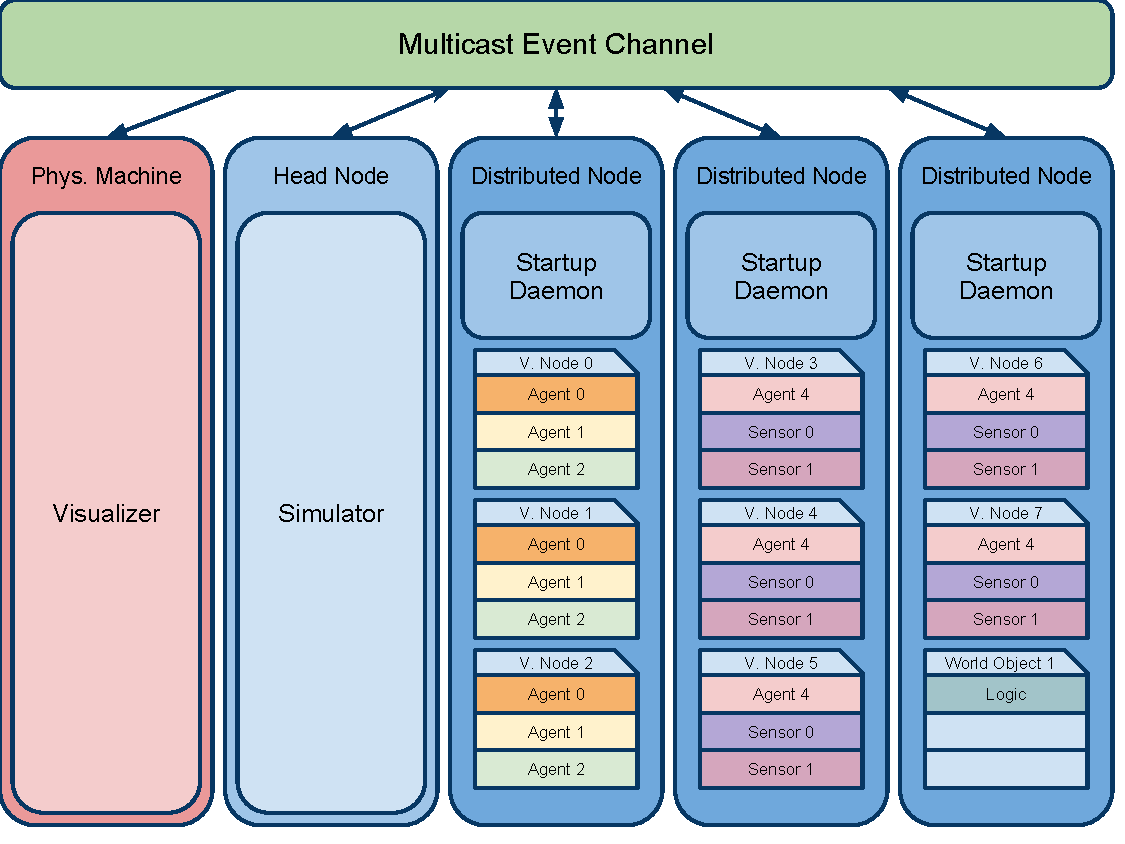
\includegraphics[scale=.6]{../initial-pres/arch.pdf}
    \caption{Distribution Diagram}
    \label{fig-distribution}
\end{figure}

\subsection{User Interface Overview}
AHOY is intentionally designed to provide no specific user interface in the traditional sense. Instead, it provides an extensive and comprehensive API, for creating a simulation, interacting with an experiment as it is running, monitoring events from a global viewpoint, and recording the results of an experiment for analysis. This ultimately offers flexibility for the end user, as separate, pre-existing interfaces can be modified to support AHOY's software API, or simply created from scratch to explicitly satisfy the user's needs. 

\subsection{Technologies Used}
The AHOY project is written entirely in Python, an interpreted, general-purpose high-level programming language. It does not depend on any external or libraries or packages, aside from those provided by the standard library. These include: the \texttt{sys} and \texttt{time} modules for standard system functions, the \texttt{math} library for advanced calculations, the \texttt{threading}, \texttt{signal} and \texttt{subprocess} for managing the distributed system, and the \texttt{pickle}, \texttt{socket} and \texttt{struct} modules for organizing the multicast event channel.

\subsection{Design Motivations}
\subsubsection{Communication}
The method by which distributed nodes communicate must provide fast, reliable, in-order delivery of event information.  Many other architectures use pair-wise TCP connections to guarantee reliability and ordered delivery, but result in significant overhead from the $n \cdot (n-1)$ connections with $n$ distributed nodes.  This results in poor scaling with large numbers of nodes.  In AHOY, a multicast event channel is used instead.

This results in no additional overhead as new distributed nodes are added.  Further, connections need not be maintained between nodes.  Due to the nature of multicast, it is possible that messages will be dropped or may arrive out of order.  However, many other frameworks, including EMANE\footnote{\url{http://labs.cengen.com/emane}} utilize multicast event channels with success.  Further, AHOY assumes all distributed nodes are running on the same subnet. In this situation, packet loss and delay is generally minimal.  In the event that messages are dropped or arrive out of order, AHOY can utilize NRL's NORM\footnote{\url{http://cs.itd.nrl.navy.mil/work/norm}} protocol which provides the same QoS guarantees as TCP.

\subsubsection{Distribution Method}
Each entity in the world, be it a node or other world object, exists as a process on one of the physical distributed nodes.  Sensors attached to each entity run as threads within that process.  Node entities may have agents running as threads also.  This model was chosen to minimize cross-machine communications as data generated from sensors need only be sent between threads of execution rather than across the event channel.  Additionally, this allows multiple agents within a single node to communicate off of the event-channel.

\section{Detailed System Design}

\subsection{Simulator Components}
\subsubsection{Simulation}
{ The Simulation starts the entire process of sending and receiving events.  It maintains the list of startup daemons running on each node. In addition, it initializes the world within the simulation along with the entities running in it. }

\attributes{
    \attribute{\_event\_api}{EventAPI}{Instance of the \texttt{EventAPI}}
    \attribute{\_startup\_acks}{list(int)}{A list of startup daemon ID's}
    \attribute{\_comms\_module}{CommsEngine}{Communication engine used to send and receive messages}
    \attribute{\_world}{World}{Instance of the world maintained by the simulation}
}

\operations{
    \operation{\_\_init\_\_(world\_inst, comms\_module)}
    {
        \begin{itemize*}
            \item \texttt{world\_inst}: Instance of the world. 
            \item \texttt{comms\_module}: Communication engine used to send and receive messages.
        \end{itemize*}
    }{None}{Instantiates the simulation}
    \operation{get\_world()}{None}{World}{Gets the \texttt{World} object being maintained}
    \operation{get\_on\_ack\_startup(event)}{Event containing the startup daemon id.}{None}{Adds a startup daemon id to the \texttt{\_startup\_acks} list}
    \operation{start(wait)}{Number of seconds to wait before starting.}{None}{Starts the simulation. Startup daemons are alerted and the \texttt{World} and the entities within it are initialized}
    \operation{stop()}{None}{None}{Stops the simulation. A \texttt{StopSimulationEvent} event is published.}
}

\subsubsection{StartupDaemon}
{Startup daemons maintain processes running on distributed nodes. It is responsible for starting and terminating these processes when appropriate.}

\attributes{
    \attribute{\_event\_api}{EventAPI}{Instance of the \texttt{EventAPI}.}
    \attribute{\_phys\_id}{int}{Integer ID assigned to the daemon.}
    \attribute{\_running\_pids}{int}{Process IDs maintained by the daemon.}
    \attribute{\_running}{bool}{True if the daemon is running.}
    \attribute{\_world}{World}{Instance of the \texttt{World} object}
}

\operations{
    \operation{\_\_init\_\_(phys\_id)}{The integer ID of the daemon.}{None}{Instantiates the \texttt{StartupDaemon}.}
    \operation{\_on\_startup(event)}{Event passed to the daemon on startup}{None}{Subscribes the daemon to the \texttt{StartSimulationEvent} and publishes an \texttt{AckStartupEvent}. It also initializes the \texttt{\_world attribute}.}
    \operation{terminate\_all()}{None}{None}{Kills all processes maintained in its list \texttt{\_running\_pids}.}
    \operation{\_start\_entity\_processes(entity)}{Entity to start and maintain.}{None}{Starts the entity passed in and adds its process ID to the list \texttt{\_running\_pids}.}
    \operation{\_on\_sim\_start(event)}{\texttt{StartSimulationEvent} published at the start of the simulation.}{None}{Gets the list of entities to maintain from \texttt{event} and calls \texttt{\_start\_entity\_process} with each one.}
    \operation{start()}{None}{None}{Starts the daemon. Subscribes to \texttt{StartupEvent} and \texttt{StopSimulationEvent} events.}
    \operation{\_restart(event)}{Event that triggered the call to \texttt{\_restart}.}{None}{Resets the state of the daemon. All processes maintained are cleared.}
    \operation{stop()}{None}{None}{Stops the daemon and sets \texttt{\_running} to false.}
}

\subsubsection{World}
{The \texttt{World} object maintains the entities running in the simulation. It also maintains the networks being used within the simulation.}

\attributes{
    \attribute{\_entities}{dict(int : Entity)}{Maps \texttt{Entity} IDs to \texttt{Entity}s}
    \attribute{\_networks}{dict(String : Network)}{Maps network names to the \texttt{Network}}
    \attribute{\_event\_api}{EventAPI}{\texttt{EventAPI} for subscribing to and publishing \texttt{Event}s}
}

\operations{
    \operation{\_\_init\_\_()}{None}{None}{Instantiates the \texttt{World}.}
    \operation{add\_entity(entity)}{Entity to be added to list of entities.}{None}{Adds an entity to \texttt{\_entities}.}
    \operation{get\_entities()}{None}{Dictionary mapping IDs to their entities.}{Returns the dictionary of entities}
    \operation{get\_entity(uid)}{Unique entity ID.}{The entity with UID \texttt{uid}.}{Returns the entity that has ID \texttt{uid}.}
    \operation{add\_network(network)}{Network to add to the dictionary of networks.}{None}{Adds the given network to the dictionary of networks. }
    \operation{get\_networks()}{None}{Dictionary mapping network names to \texttt{Network} instances.}{Returns the dictionary of networks}
    \operation{get\_network(name)}{Name of the network.}{Gets the network with name \texttt{name}.}{Returns the network whose name is the same as the parameter}
    \operation{initialize()}{None}{None}{Initializes the \texttt{World}. Instantiates \texttt{\_event\_api}, starts it, and subscribes the \texttt{World} to events.}
    \operation{\_on\_entity\_move(event)}{\texttt{EntityMoveEvent} event with information on new entity values.}{None}{Finds the entity in \texttt{\_entities} given by the event and updates that entity's position and velocity.}
    \operation{pickle()}{None}{Serialized version of the \texttt{World} object.}{Serializes the \texttt{World}.}
    \operation{from\_pickle(pickled)}{Serialized version of the \texttt{World} object.}{\texttt{World} object}{De-serializes a pickled version of the \texttt{World} object.}
}
    
\subsubsection{EventAPI}
{The \texttt{EventAPI} is used to communicate events across the event channel. It allows entities to subscribe to certain events or publish the occurrence of events. When an event occurs, it will handle any function calls an entity wishes to make during that event.}

\attributes{
    \attribute{\_subscriptions}{dictionary}{Holds event subscriptions for an entity. Keyed by event type. The values are method calls to be made on an event.}
    \attribute{\_running}{bool}{True if the \texttt{EventAPI} is running.}
    \attribute{\_tcp\_conn}{socket}{An optional TCP socket that will be used instead of the multicast channel to access the \texttt{EventAPI}}
    \attribute{\_sock}{socket}{A socket for \texttt{EventAPI} to communicate over}
    \attribute{\_ip}{string}{IP address to communicate on}
    \attribute{\_port}{int}{Port number to communicate on}
}

\operations{
    \operation{\_\_init\_\_(tcp\_conn)}{A socket for the \texttt{EventAPI} to communicate over}{None}{Instantiates an \texttt{EventAPI}}
    \operation{\_setup\_mc()}{None}{None}{Initializes the multicast channel to communicate on.}
    \operation{publish(event,delay\_sec)}
    {
        \begin{itemize*}
            \item \texttt{event}: The event to be published. 
            \item \texttt{delay}: Number of seconds to wait before publishing. 
        \end{itemize*}
    }{None}{Publishes the occurrence of an event over the event channel.}
    \operation{\_delay(event, delay\_sec)}
    {
        \begin{itemize*}
            \item \texttt{event}: The event to delay.
            \item \texttt{delay\_sec}: Number of seconds to delay the event. 
        \end{itemize*}
    }{None}{Delays an event for a given number of seconds.}
    \operation{push\_raw(raw)}{Data to send over a connection.}{None}{Sends raw data over the current connection.}
    \operation{subscribe(event\_type, callback, **args)}
    {
        \begin{itemize*}
            \item \texttt{event\_type}: Event type being subscribed to. 
            \item \texttt{callback}: Method to call on \texttt{event\_type}.
            \item \texttt{**args}: arguments to pass to callback.
        \end{itemize*}
    }{None}{Sets a callback function to be made at a given event type.}
    \operation{unsubscribe\_all(event\_type)}{The type of event to remove all subscriptions from.}{None}{Removes all subscriptions to the given event type.}
    \operation{clear\_subscriptions()}{None}{None}{Removes all subscriptions.}
    \operation{\_process(data)}{Serialized event information.}{None}{Processes which callbacks need to be made based on the given data.}
    \operation{run()}{None}{None}{Listens for events over the socket and processes them.}
    \operation{\_tcp\_assemble()}{None}{Packet}{Builds a packet to be sent over the network.}
    \operation{start()}{None}{Thread}{Runs the \texttt{EventAPI} in a thread and returns the thread.}
    \operation{stop()}{None}{None}{Stops the \texttt{EventAPI} from running. }
}
    
\subsubsection{Entity}
\attributes{
    \attribute{MAX\_DISTANCE}{const float}{Maximum distance the entity can move in kilometers before publishing a move event.}
    \attribute{\_uid}{int}{Unique user id of the entity.}
    \attribute{\_lat}{float}{Current latitude.}
    \attribute{\_long}{float}{Current longitude.}
    \attribute{\_agl}{float}{Distance above ground level.}
    \attribute{\_rcs}{float}{Approximate cross-sectional area.}
    \attribute{\_event\_api}{EventAPI}{The \texttt{EventAPI} for an entity.}
    \attribute{\_world}{World}{The World instance.}
    \attribute{\_velocity}{\texttt{list(float)}}{The vector velocity of the entity.}
    \attribute{\_forward\_velocity}{float}{The forward velocity of the entity.}
    \attribute{\_sensors}{dict(String : Sensor)}{Sensors connected to the entity.}
}

\operations{
    \operation{add\_sensor(name, sensor)}
    {
        \begin{itemize*}
            \item \texttt{name}: Name of the sensor.
            \item \texttt{sensor}: Sensor instance
        \end{itemize*}
    }{None}{Adds a sensor and associates it with a name.}
    \operation{get\_sensor(name)}{Name of the sensor}{Sensor instance}{Gets a sensor by name.}
    \operation{set\_rcs(rcs)}{Cross sectional-area}{None}{Sets the cross-sectional area.}
    \operation{get\_rcs()}{None}{Cross-sectional area}{The cross-sectional area.}
    \operation{get\_velocity()}{None}{A tuple of the velocity vectors}{Returns the velocity as a vector of three numbers.}
    \operation{set\_velocity(v)}{A vector of three floating point numbers describing the velocity.}{None}{Sets the vector velocity of the entity.}
    \operation{set\_world(world)}{The \texttt{World} instance}{None}{Sets the \texttt{World} instance for the entity}
    \operation{get\_world()}{None}{A \texttt{World} instance}{Returns the \texttt{World} instance.}
    \operation{set\_position(lat,long,agl)}
    {
        \begin{itemize*}
            \item \texttt{lat}: Latitude to assign the entity. 
            \item \texttt{long}: Longitude to assign the entity. 
            \item \texttt{agl}: Above ground location to assign the entity. 
        \end{itemize*}
    }{None}{Sets the latitude, longitude, and above ground location for the entity.}
    \operation{move(lat,lon,agl,forward\_vel,vert\_vel,block=False)}
    {
        \begin{itemize*}
            \item \texttt{lat}: Latitude to move to.
            \item \texttt{lon}: Longitude to move to.
            \item \texttt{agl}: Above ground location to move to. 
            \item \texttt{forward\_vel}: Forward velocity to move with.
            \item \texttt{vert\_vel}: Vertical velocity to move with. 
            \item \texttt{block}: If true, moves the entity in a new thread.
        \end{itemize*}
    }{None}{Moves the entity to the given coordinates.}
    \operation{\_iterative\_move(lat,lon,agl,forward\_vel,vert\_vel)}
    {
        \begin{itemize*}
            \item \texttt{lat}: Latitude to move to.
            \item \texttt{lon}: Longitude to move to.
            \item \texttt{agl}: Above ground location to move to. 
            \item \texttt{forward\_vel}: Forward velocity to move with.
            \item \texttt{vert\_vel}: Vertical velocity to move with. 
        \end{itemize*}
    }{None}{Moves the entity to the given coordinates in steps by smaller distances.}
    \operation{get\_position()}{None}{A tuple containing lat, lon and agl}{Returns a list of the latitude, longitude, and above ground location in that order.}
    \operation{pickle()}{None}{Serialized Entity}{Serializes the entity.}
    \operation{from\_pickle(pickled)}{A serialized \texttt{Entity}.}{An \texttt{Entity} object}{De-serializes an entity.}
    \operation{get\_event\_api()}{None}{An \texttt{EventAPI} instance}{Returns the entity's \texttt{EventAPI}.}
    \operation{get\_uid()}{None}{ID of the \texttt{Entity} instance}{Returns the entity's unique ID.}
    \operation{initialize()}{None}{None}{Initializes the \texttt{Entity}.}
}
\begin{figure}[!htb]
  \centering

  \begin{sequencediagram}{3cm}
    \newthread{ent}{Entity}{Entity}
    \newthread{ec}{Event Channel}{Event Channel}
    \newthread{all}{World Instances}{World Instances}

    \begin{sdloop}{loop [not at dest]}
        \begin{callself}{ent}{\_iterate\_move()}{}
            \mess{ent}{EntityMoveEvent}{ec}
            \mess{ec}{EntityMoveEvent}{all}
            \begin{callself}{all}{\_on\_entity\_move()}{}
            \end{callself}
        \end{callself}
    \end{sdloop}
  \end{sequencediagram}

  \caption{Movement iteration}
  \label{fig-movement}
\end{figure}

\subsubsection{Built-in Entities}
\paragraph{Node}{Nodes are processes that aggregate agents. Each one has an interface that handles communication to the outside world (i.e. other nodes or agents). They inherit properties from the Entity class.}

\attributes{
    \attribute{\_interfaces}{dict(String : Interface)}{A dictionary mapping the name of an network interface to the interface itself. }
    \attribute{\_agents}{dict(int : Agent)}{A dictionary mapping agent IDs to the agents themselves.}
}

\operations{
    \operation{\_\_init\_\_(uid)}{Unique ID assigned to the node.}{None}{Instantiates the \texttt{Node}.}
    \operation{get\_agent\_uids()}{None}{A list of the agent UIDs}{Returns a list of all agent IDs belonging to that node.}
    \operation{add\_interface(interface)}{Network interface to add to the node.}{None}{Adds a network interface to the node.}
    \operation{remove\_interface(name)}{The name of the interface to remove.}{None}{Removes an network interface from the node.}
    \operation{get\_interface(name)}{The name of the interface to return.}{Interface}{Returns a network interface with the given name.}
    \operation{get\_interfaces()}{None}{A list of network interfaces}{Returns a list of all network interfaces belonging to the node.}
    \operation{add\_agent(agent\_inst)}{Agent to add to the node.}{None}{Adds an agent to the list of agents owned by the node.}
    \operation{get\_interface\_on\_net(network\_name)}{Network name associated with an interface.}{None}{Returns the interface associated with the given network name.}
    \operation{send(message,src\_agent)}
    {
        \begin{itemize*}
            \item \texttt{message}: Message to send. 
            \item \texttt{src\_agent} Agent sending the message.
        \end{itemize*}
    }{None}{Sends a message from a specified agent over a node interface.}
    \operation{\_on\_message(event,**kwds)}
    {
        \begin{itemize*}
            \item \texttt{event}: An event that has occurred. 
            \item \texttt{**kwds}: Arguments associated with the callback for an event.
        \end{itemize*}
    }{None}{Passes an event on to the agent it is meant to reach.}
    \operation{run()}{None}{None}{Starts the node. Interfaces and agents are all initialized}
}

\paragraph{ScriptedEntity}{An entity that moves based on a pre-scripted mobility plan.}

\attributes
{
    \attribute{\_waypoints}{list((lat, lon, agl))}{Waypoints to follow.}
    \attribute{\_vel}{float}{Velocity with which the entity should move.}
}

\operations
{
    \operation{\_\_init\_\_(uid, waypoints, vel)}{
        \begin{itemize*}
            \item \texttt{uid}: Unique ID for the entity.
            \item \texttt{waypoints}: Waypoints to follow.
            \item \texttt{vel}: Velocity of movement
        \end{itemize*}
    }{None}{Instantiates a \texttt{ScriptedEntity} which will move along a specified set of waypoints at a specific velocity.}
    \operation{run()}{None}{None}{Starts the entity.}
}

\subsubsection{Startup Sequence}
As shown in Figure~\ref{fig-startupseq}, the startup sequence for a simulation is comprised of three major steps.  Initially, the \texttt{Simulation} process publishes a \texttt{StartupEvent}, which results in all \texttt{StartupDaemon} processes responding with an \texttt{AckStartupEvent}.  These acknowledgements are then used by the \texttt{Simulation} to equally distribute \texttt{Entities} across the daemons.  This distribution is communicated with a \texttt{SimulationStartEvent} which contains a list of entities to bestarted on each daemon.  Additionally, this causes all daemons to start the simulation.
\begin{figure}[!htb]
  \centering

  \begin{sequencediagram}{3.5cm}
    \newthread{sim}{Simulation}{Simulation}
    \newthread{mc}{Event Channel}{EventChannel}
    \newthread{startup1}{StartupDaemon 1}{StartupDaemon}
    \newthread{startupn}{StartupDaemon $n$}{StartupDaemon}

    \mess{sim}{StartupEvent}{mc}
    \begin{callself}{sim}{time.sleep()}{}
        \mess{mc}{StartupEvent}{startup1}
        \mess{mc}{\hspace*{3cm}StartupEvent}{startupn}
        \mess{startup1}{AckStartupEvent}{mc}
        \mess{mc}{AckStartupEvent}{sim}
        \mess{startupn}{\hspace*{3cm}AckStartupEvent}{mc}
        \mess{mc}{AckStartupEvent}{sim}
    \end{callself}
    \begin{callself}{sim}{allocate\_entities()}{}
    \end{callself}
    \mess{sim}{StartSimulationEvent}{mc}
    \mess{mc}{StartSimulationEvent}{startup1}
    \begin{callself}{startup1}{start\_entities()}{}
    \end{callself}
    \mess{mc}{\hspace*{3.7cm}StartSimulationEvent}{startupn}
    \begin{callself}{startupn}{start\_entities()}{}
    \end{callself}
  \end{sequencediagram}

  \caption{Startup sequence}
  \label{fig-startupseq}
\end{figure}
\subsection{Networking Components}
\begin{figure}[!htb]
    \centering

    \begin{sequencediagram}{4cm}
        \newthread{node}{Node}{Node}
        \newthread{mc}{Event Channel}{Event Channel}
        \newthread{ce}{CommsEngine}{CommsEngine}

        \mess{node}{CommunicationSendEvent}{mc}
        \mess{mc}{CommunicationSendEvent}{ce}
        \begin{callself}{ce}{\_on\_send}{}
        \end{callself}
        \begin{sdloop}{alt [send successful]}
            \mess{ce}{CommunicationRecvEvent}{mc}
            \mess{mc}{CommunicationRecvEvent}{node}
        \end{sdloop}
    \end{sequencediagram}

    \caption{Messaging sequence diagram}
    \label{fig-messageseq}
\end{figure}

\subsubsection{Interface}

\attributes{
    \attribute{\_name}{String}{The name of the \texttt{Interface}}
    \attribute{\_owner}{Node}{The \texttt{node} on which the \texttt{Interface} resides}
    \attribute{\_recv\_callback}{function}{The callback function}
    \attribute{\_network\_name}{String}{The name of the \texttt{Network}}
    \attribute{\_power}{float}{The power of the interface, if a wireless network}
}

\operations{
    \operation{\_\_init\_\_(name, owner\_node, network, power)}
    {
        \begin{itemize*}
            \item \texttt{name}: The name of the \texttt{Interface} 
            \item \texttt{owner\_node}: The \texttt{Node} on which the \texttt{Interface} resides
            \item \texttt{network}: The \texttt{Network} to which the \texttt{Interface} belongs
            \item \texttt{power}: The power of the \texttt{Interface}, if wireless.
        \end{itemize*}
    }{None}{Sends a given message from the specified agent}
    \operation{connect()}{None}{None}{Connects the \texttt{Interface} to the \texttt{Network}}
    \operation{send(message\_inst, src\_agent)}
    {
        \begin{itemize*}
            \item \texttt{message\_inst}: The \texttt{Message} that is being sent on the \texttt{Interface}
            \item \texttt{src\_agent}: The \texttt{Agent} which is sending the \texttt{Message}
        \end{itemize*}
    }{None}{Sends a given message from the specified agent}
    \operation{set\_recv\_callback(cb)}{The callback function}{None}{Sets the callback function for the interface}
    \operation{get\_owner()}{None}{The \texttt{Node} which is the owner of the \texttt{Interface}}{Returns the \texttt{Node} which is the owner of the \texttt{Interface}}
    \operation{get\_network\_name()}{None}{The name of the \texttt{Network} the \texttt{Interface} is part of}{Returns the name of the \texttt{Network} the \texttt{Interface} is part of}
    \operation{get\_name()}{None}{The name of the \texttt{Interface}}{Returns the name of the interface}
    \operation{get\_power()}{None}{The power of the \texttt{Interface}}{Returns the power of the interface}
}

\subsubsection{CommsEngine}

\attributes{
    \attribute{\_event\_api}{EventAPI}{The \texttt{EventAPI} instance}
    \attribute{\_simulation}{Simulation}{The \texttt{Simulation} instance}
}

\operations{
    \operation{\_\_init\_\_()}{None}{None}{Initializes the \texttt{CommsEngine}}
    \operation{get\_node\_from\_agent(agent\_uid)}{The UID of the \texttt{Agent}}{An \texttt{Agent} instance}{Returns the \texttt{Agent} with the given UID}
    \operation{set\_simulation(simulation)}{An instance of the \texttt{Simulation}}{None}{Sets the \texttt{CommsEngine}'s \texttt{Simulation} instance}
    \operation{get\_event\_api()}{None}{An \texttt{EventAPI} instance}{Returns an instance of the \texttt{EventAPI}}
    \operation{get\_simulation()}{None}{An \texttt{Simulation} instance}{Returns an instance of the \texttt{Simulation}}
    \operation{\_on\_send(event)}{An \texttt{Event}}{None}{Abstract method which is invoked whenever a node transmits a message.}
}

\subsubsection{Built-in CommsEngines}
\paragraph{LogLossCommsEngine}{Provides basic log-loss model for communications.  When messages are sent on a wireless network, the received power is calculated with:

\begin{align*}
    P_r = P_t - \left(l_0 - 10 \cdot \gamma \cdot log_{10}\left(\frac{d}{d_0}\right) + X_g\right)
\end{align*}

where $P_t$ is the transmit power, $\gamma$ is a path-loss exponent, $d_0$ is an arbitrary reference distance, $l_0$ is the loss at that distance, $d$ is the actual distance between the two interfaces, and $X_g$ is a constant accounting for flat-fading.  If this power falls below the sensitivity of the receiver, the message will not be received.}

\noattributes

\operations
{
    \operation{\_\_init\_\_()}{none}{none}{instantiates a new \texttt{loglosscommsengine}.}
    \operation{\_get\_rx\_power(src\_uid, dest\_uid, src\_power}{
        \begin{itemize*}
            \item \texttt{src\_uid}: uid of transmitting node.
            \item \texttt{dest\_uid}: uid of destination node.
            \item \texttt{src\_power}: power of transmitter.
        \end{itemize*}}{the received power in watts.}{calculates the pathloss between two nodes.}
    \operation{\_should\_deliver(src\_uid, dest\_uid, src\_power, recv\_sensitivity)}{
        \begin{itemize*}
            \item \texttt{src\_uid}: uid of transmitting node.
            \item \texttt{dest\_uid}: uid of destination node.
            \item \texttt{src\_power}: power of transmitter.
            \item \texttt{recv\_sensitivity}: receiver sensitivity.
        \end{itemize*}}{bool}{determines if the link between two nodes is strong enough to deliver messages.  calls \texttt{\_get\_rx\_power()} for pathloss.}
    \operation{\_on\_send(event)}{instance of \texttt{communicationsendevent}}{none}{determines what occurs when a node transmits a message.}
    \operation{\_on\_movement(event)}{instance of \texttt{entitymoveevent}}{none}{updates links based on new node locations.}
}

\paragraph{EthernetCommsEngine}{Provides basic support for Ethernet communications.}

\noattributes

\operations
{
    \operation{\_\_init\_\_()}{None}{None}{Instantiates a new \texttt{EthernetCommsEngine}.}
    \operation{\_on\_send(event)}{Instance of \texttt{CommunicationSendEvent}}{None}{Determines what occurs when a node transmits a message.}
}

\subsection{Event Components}
\subsubsection{Event}{Event is the base abstract class from which all other events descend.  This class provides picking and un-pickling methods used to send events over the event channel.}

\noattributes

\operations
{
    \operation{\_\_init\_\_()}{None}{None}{Instantiates a new event.}
    \operation{pickle()}{None}{Serialized World}{Serializes the \texttt{Event}.}
    \operation{from\_pickle(pickled)}{Serialized version of the \texttt{Event} object.}{\texttt{Event} object}{De-serializes a pickled version of the \texttt{Event} object.}
}

\subsubsection{Built-in Events}
Built-in events are specific Event classes provided by default to any emulation. These embody the basic events for a network simulation, but users are encouraged to develop and add their own as well.
\paragraph{LinkEvent}{Published when a network link between two entities' changes within the simulation.}

\attributes{
    \attribute{\_up}{bool}{Whether the link is currently up (connected)}
    \attribute{\_uid\_1}{int}{UID of the first node which makes up the link}
    \attribute{\_uid\_2}{int}{UID of the second node which makes up the link}
    \attribute{\_network\_name}{string}{The network that the link exists on}
    \attribute{\_pathloss}{float}{Pathloss value for wireless links}
}

\operations{
    \operation{\_\_init\_\_(up, uid\_1, uid\_2, network\_name, pathloss)}
    {
        \begin{itemize*}
            \item \texttt{up}: Whether the link is up
            \item \texttt{uid\_1}: The UID of the first node
            \item \texttt{uid\_2}: The UID of the second node
            \item \texttt{network\_name}: The name of the network
            \item \texttt{pathloss}: The pathloss value, if relevant
        \end{itemize*}
    }{None}{Instantiates a new link action}
    \operation{get\_up()}{None}{Link State}{Gets whether or not the link is connected}
    \operation{get\_uid1()}{None}{First Agent UID}{Gets the UID of the first node in the link}
    \operation{get\_uid2()}{None}{Second Agent UID}{Gets the UID of the second node in the link}
    \operation{get\_network\_name()}{Network Name}{None}{Gets the name of the network}
    \operation{get\_pathloss()}{None}{Pathloss Value}{Gets the pathloss value for wireless links}
}

\paragraph{CommunicationSendEvent}{Published when an entity sends a message within the simulation.}

\attributes{
    \attribute{\_src\_agent\_uid}{int}{UID of the entity that is the source of the message}
    \attribute{\_src\_iface\_name}{string}{Interface name that the message is sent on}
    \attribute{\_message}{Message}{An instance of the message that is sent}
    \attribute{\_network}{string}{The network that the interface is a part of}
}

\operations{
    \operation{\_\_init\_\_(src\_agent\_uid, src\_iface\_name, message\_inst, network)}
    {
        \begin{itemize*}
            \item \texttt{src\_agent\_uid}: UID of the sending agent
            \item \texttt{src\_iface\_name}: Name of the interface
            \item \texttt{message\_inst}: Instance of the message being sent
            \item \texttt{network}: Name of the network
        \end{itemize*}
    }{None}{Instantiates a new communication send action}
    \operation{get\_src\_agent\_uid()}{None}{Source Agent UID}{Gets the UID of the source entity that sent the message}
    \operation{get\_src\_iface\_name()}{None}{Source Interface Name}{Gets the name of the interface the message was sent on}
    \operation{get\_message()}{None}{Message}{Gets the entirety of the message}
    \operation{get\_network()}{None}{Network Name}{Gets the network the message was sent on}
}

\paragraph{CommunicationRecvEvent}{Published when an entity receives a message within the simulation.}

\attributes{
    \attribute{\_src\_agent\_uid}{int}{UID of the entity that is the source of the message}
    \attribute{\_src\_iface\_name}{string}{Interface name that the message is sent on}
    \attribute{\_message}{Message}{An instance of the message that is sent}
    \attribute{\_network}{string}{The network that the interface is a part of}
}

\operations{
    \operation{\_\_init\_\_(src\_agent\_uid, src\_iface\_name, message\_inst, network)}
    {
        \begin{itemize*}
            \item \texttt{src\_agent\_uid}: UID of the sending agent
            \item \texttt{src\_iface\_name}: Name of the interface
            \item \texttt{message\_inst}: Instance of the message being sent
            \item \texttt{network}: Name of the network
        \end{itemize*}
    }{None}{Instantiates a new communication receive action}
    \operation{get\_src\_agent\_uid()}{None}{Source Agent UID}{Gets the UID of the source entity that sent the message}
    \operation{get\_src\_iface\_name()}{None}{Source Interface Name}{Gets the name of the interface the message was sent on}
    \operation{get\_message()}{None}{Message}{Gets the entirety of the message}
    \operation{get\_network()}{None}{Network Name}{Gets the network the message was sent on}
}

\paragraph{EntityMoveEvent}{Published when an entity moves within the simulation.}

\attributes{
    \attribute{\_entity\_uid}{int}{UID of the entity that moved}
    \attribute{\_lat}{float}{Latitude of new location}
    \attribute{\_lon}{float}{Longitude of new location}
    \attribute{\_agl}{float}{AGL of new location}
    \attribute{\_velocity}{float}{Velocity of movement}
}

\operations
{
    \operation{\_\_init\_\_(entity, lat, lon, agl, velocity)}
    {
        \begin{itemize*}
            \item \texttt{entity}: Instance of entity that moved
            \item \texttt{lat}: Latitude of new location
            \item \texttt{lon}: Longitude new location
            \item \texttt{agl}: AGL of new location
            \item \texttt{velocity}: Velocity of movement
        \end{itemize*}
    }{None}{Instantiates a new movement action}
    \operation{get\_uid()}{None}{UID}{Gets the UID of the entity that moved}
    \operation{get\_lat()}{None}{Latitude}{Gets the new latitude of the entity that moved}
    \operation{get\_lon()}{None}{Longitude}{Gets the new longitude of the entity that moved}
    \operation{get\_agl()}{None}{AGL}{Gets the new AGL of the entity that moved}
    \operation{get\_velocity()}{None}{Velocity}{Gets the velocity of the entity that moved}
}

\paragraph{StartupEvent}{Event requesting all daemons on the event channel to respond with their IDs.  Further, a \texttt{World} instance is sent out which stored by the daemons until a \texttt{StartSimulationEvent} is received.}
\attributes
{
    \attribute{\_world}{World}{Instance of the \texttt{World} to be used in the simulation.}
}

\operations
{
    \operation{\_\_init\_\_(world)}{Instance of the world to be used in the simulation.}{None}{Instantiates a new \texttt{StartupEvent}.}
    \operation{get\_world()}{None}{\texttt{World} instance to be used in the simulation.}{Gets the world instance which will be used after \texttt{StartSimulationEvent} is received.}
}

\paragraph{AckStartupEvent}{Event published by all daemons in response to a \texttt{StartupEvent}.  Allows the simulation to allocate entities equally.}
\attributes
{
    \attribute{\_daemon\_id}{int}{ID of the daemon which sent the ACK.}
}

\operations
{
    \operation{\_\_init\_\_(daemon\_id)}{ID of the daemon.}{None}{Instantiates a new \texttt{AckStartupEvent}.}
    \operation{get\_daemon\_id()}{None}{ID of the ACK-ing daemon.}{Gets the ID of the ACK-ing daemon.}
}

\paragraph{StartSimulationEvent}{Event used to trigger a simulation to begin.  Issuing this allocates entities across daemons.}
\attributes
{
    \attribute{\_entity\_mapping}{dict(int : int)}{Mapping of daemon IDs to entity IDs.}
}

\operations
{
    \operation{\_\_init\_\_(entity\_mapping)}{Daemon to entity ID mapping.}{None}{Instantiates a new \texttt{StartSimulationEvent}.}
    \operation{get\_mapping()}{None}{Mapping of daemon IDs to entity IDs.}{Daemons receive this event and start only the entities which they have been allocated.}
}

\paragraph{StopSimulationEvent}{An event that stops the simulation.  All simulation state information on daemons is reset.}

\noattributes

\operations
{
    \operation{\_\_init\_\_()}{None}{None}{Instantiates a new \texttt{StopSimulationEvent}.}
}

\subsection{Agent Components}
\subsubsection{Agent}
{An \texttt{Agent} is an intelligent algorithm that makes decisions based on data it receives from its environment and its beliefs about the current state of the system. \texttt{Agent}s are run as threads on distributed nodes. }

\attributes{
    \attribute{\_owner\_node}{\texttt{Node}}{Node that owns the \texttt{Agent}}
    \attribute{\_uid}{int}{Unique identifier.}
    \attribute{\_behaviors}{dict(entity : [\texttt{Condition},\texttt{Action}])}{Behavior map linking \texttt{Event}s to \texttt{Action}s.}
}

\operations{
    \operation{get\_uid()}{None}{The \texttt{Agent}'s UID}{Returns the unique ID.}
    \operation{get\_owner\_node()}{None}{The \texttt{Node} on which this \texttt{Agent} is running}{Returns the node that owns the agent.}
    \operation{start()}{None}{A thread}{Returns the \texttt{Agent} thread.}
    \operation{on\_message(event)}{An instance of a \texttt{CommunicationRecvEvent} containing a \texttt{Message}.}{None}{Abstract method for handling message events.}
    \operation{run()}{None}{None}{Abstract method for starting the \texttt{Agent} thread.}
    \operation{add\_behavior(behavior)}{A behavior tuple in the form (\texttt{Condition}, \texttt{Event}, \texttt{Action})}{None}{Adds a behavior tuple to the \texttt{Agent}.}
    \operation{remove\_behavior(behavior)}{A behavior tuple in the form (\texttt{Condition}, \texttt{Event}, \texttt{Action})}{None}{Removes the specified behavior tuple.}
    \operation{\_on\_event(event)}{An \texttt{Event} which may result in an \texttt{Action}.}{None}{Performs an \texttt{Action} based on the \texttt{Event} and \texttt{Condition} associated with it.}
    \operation{\_init\_behaviors()}{None}{None}{Initializes the \texttt{Agent} behaviors.}
}

\subsubsection{Condition}
{A \texttt{Condition} is an abstract class used to determine if some state in the system is true or false. It is used by an \texttt{Agent} to decide if it should perform an \texttt{Action}.}

\noattributes{}

\operations{
    \operation{\_\_init\_\_()}{None}{None}{Initializes the abstract \texttt{Condition}.}
    \operation{is\_met(event)}{An \texttt{Event}}{None}{Abstract method for testing if the \texttt{Condition} is true or not.}
}

\subsubsection{Action}
{An \texttt{Action} is an abstract class that allows an \texttt{Agent} to perform a specific task.  All user defined and built in actions inherit this base class.}

\noattributes{}

\operations{
    \operation{\_\_init\_\_()}{None}{None}{Initializes the abstract \texttt{Action} class.}
    \operation{perform()}{None}{None}{Abstract method for performing the \texttt{Action}.}
}

\subsubsection{Built-in Actions}
\paragraph{MoveAction}
{\texttt{MoveAction} moves an entity to a specified location. It is used by an \texttt{Agent}.}

\attributes{
    \attribute{\_lat\_move}{float}{The latitude to move to.}
    \attribute{\_lon\_move}{float}{The longitude to move to.}
    \attribute{\_alt\_move}{float}{The above ground location to move to.}
    \attribute{\_entity}{\texttt{Entity}}{The \texttt{Entity} to move.}
}

\operations{
    \operation{\_\_init\_\_(node,lat,lon,alt)}
    {
        \begin{itemize*}
            \item \texttt{node}: The \texttt{Entity} being moved. 
            \item \texttt{lat}: The latitude to move to. 
            \item \texttt{lon}: The longitude to move to. 
            \item \texttt{alt}: The above ground location to move to. 
        \end{itemize*}
    }{None}{Initializes the \texttt{MoveAction} class.}
    \operation{perform()}{None}{None}{Moves \_entity to the position given at initialization.}
}

\subsection{Sensor Components}
\subsubsection{Sensor}
\attributes
{
    \attribute{\_subscribers}{list(function)}{List of functions to call when the sensor has new data.}
}

\operations
{
    \operation{\_publish\_data(event)}{An event containing data to publish.}{None}{Called by the sensor to pass new data to all callbacks}
    \operation{subscribe(callback)}{A callback function.}{None}{Subscribes to the sensor.  Any time new data is available, \texttt{callback} will be invoked and passed the data.}
    \operation{run()}{None}{None}{Abstract method.  Called to start the sensor.}
}

\subsubsection{Built-in Sensors}
\paragraph{RadarSensor}{AHOY includes a Radar sensor which provides an estimated location of nearby entities along with velocity estimation.  This sensor sweeps angular areas surrounding it and calculates the distance to the closest entity in that area with:
\begin{align*}
    d = \frac{t \cdot c}{2}
\end{align*}

Based on the latitude ($\phi_r$) and longitude ($\lambda_r$) of the radar sensor, along with the bearing $\theta$ of the sweep area, the entity's location $\left(\phi_t, \lambda_t\right)$ can be estimated with:
\begin{align*}
    \phi_t &=& sin^{-1}\left(sin\left(\phi_r\right) \cdot cos\left(d/R_{e}\right) + cos\left(\phi_r\right) \cdot sin\left(d/R_{e}\right) \cdot cos\left(\theta\right)\right) \\ 
    \lambda_t &=& \lambda_t + tan^{-1}\left(sin\left(\theta\right) \cdot sin\left(d/R_{e}\right) \cdot cos\left(\phi_r\right), cos\left(d/R_{e}\right)-sin\left(\phi_r\right) \cdot sin\left(\phi_t\right)\right)
\end{align*}

An estimate of velocity\footnote{Specifically, the component of the velocity parallel to the vector from the radar sensor to the entity} is calculated by the Doppler equation:

\begin{align*}
    \left|\vec{v_{\parallel}}\right| = -\frac{c \cdot \left(f_{recv} - f_{trans}\right)}{f_{trans}}.
\end{align*}

Further, pathloss of radio waves is incorporated. The received power, $P_r$, to the radar sensor is given by:

\begin{align*}
    P_r = \frac{P_t G_t A_r \sigma F^4}{\left(4 \pi\right)^4 d^4}
\end{align*}

where $P_t$ is the transmit power, $G_t$ is the antenna gain, $A_r$ is the aperture area, $\sigma$ is the cross-sectional area of the target, $F$ is a propagation factor, and $d$ is the distance from the radar station to the target.  If $P_r$ falls below the sensitivity of the antenna, the target will not be detected.
}

\attributes
{
    \attribute{\_trans\_power}{float}{Transmit power of the Radar.}
    \attribute{\_trans\_freq}{float}{Frequency of the Radar.}
    \attribute{\_gain}{float}{Gain of the Radar.}
    \attribute{\_aperture}{float}{Aperture of the Radar.}
    \attribute{\_prop\_fact}{float}{Propagation factor of the environment.}
    \attribute{\_angle}{float}{Sweep angle of the Radar.}
    \attribute{\_dwell\_time}{float}{Time spent sweeping each \texttt{\_angle}.}
}

\operations
{
    \operation{\_\_init\_\_(trans\_power, trans\_freq, gain, aperture, prop\_fact, dwell\_time, angle)}{
        \begin{itemize*}
            \item \texttt{trans\_power}: Transmit power of the Radar.
            \item \texttt{trans\_freq}: Frequency of the Radar.
            \item \texttt{gain}: Gain of the Radar.
            \item \texttt{aperture}: Aperture of the Radar.
            \item \texttt{prop\_fact}: Propagation factor of the environment.
            \item \texttt{angle}: Sweep angle of the Radar.
            \item \texttt{dwell\_time}: Time spent sweeping each \texttt{\_angle}.
        \end{itemize*}}{None}{Instantiates a new \texttt{RadarSensor}.}
    \operation{run()}{None}{None}{Starts the Radar.}
}

\subsection{Utility Components}
\subsubsection{Geo}

\noattributes

\operations{
    \operation{haver\_distance(lat1, lon1, lat2, lon2)}
    {
        \begin{itemize*}
            \item \texttt{lat1}: Latitude of first point
            \item \texttt{lon1}: Longitude of first point
            \item \texttt{lat2}: Latitude of second point
            \item \texttt{lon2}: Longitude of second point
        \end{itemize*}
    }{Haversine distance between two points}{Determines the ``as-the-bird-flies'' distance between to points.}
    \operation{linear\_distance(lat1, lon1, lat2, lon2)}
    {
        \begin{itemize*}
            \item \texttt{lat1}: Latitude of first point
            \item \texttt{lon1}: Longitude of first point
            \item \texttt{lat2}: Latitude of second point
            \item \texttt{lon2}: Longitude of second point
        \end{itemize*}
    }{Linear distance between two points}{Determines the linear distance between two points.}
    \operation{sph\_to\_lin(lat, lon, agl)}
    {
        \begin{itemize*}
            \item \texttt{lat}: Latitude of point
            \item \texttt{lon}: Longitude of point
            \item \texttt{agl}: AGL of point
        \end{itemize*}
    }{\texttt{(x,y,z)} tuple of location}{Converts latitude, longitude, and altitude into Cartesian coordinates.}
    \operation{lin\_to\_sph(x, y, z)}
    {
        \begin{itemize*}
            \item \texttt{x}: $x$-coordinate of point
            \item \texttt{y}: $y$-coordinate of point
            \item \texttt{z}: $z$-coordinate of point
        \end{itemize*}
    }{\texttt{(lat, lon, agl)} tuple of location}{Converts Cartesian coordinates into latitude, longitude, and altitude.}
    \operation{lin\_to\_degree(lat, lon, lat\_km, lon\_km)}
    {
        \begin{itemize*}
            \item \texttt{lat}: Latitude of point
            \item \texttt{lon}: Longitude of point
            \item \texttt{lat\_km}: Kilometers along latitude line
            \item \texttt{lon\_km}: Kilometers along longitude line
        \end{itemize*}
    }{Radians of movement}{Converts distance in kilometers to radians at a given point on the Earth.}
    \operation{loc\_from\_bearing\_dist(lat, lon, bearing, dist)}
    {
        \begin{itemize*}
            \item \texttt{lat}: Latitude of point
            \item \texttt{lon}: Longitude of point
            \item \texttt{bearing}: Bearing of movement
            \item \texttt{dist}: Distance of movement in kilometers
        \end{itemize*}
    }{\texttt{(lat, lon)} tuple of new location}{Determines location after moving from a point, along a bearing, for a specific distance.}
}
\pagebreak
\section{Appendix}
\subsection{UML Class Diagrams}
\begin{figure}[!ht]
    \centering
    \begin{tikzpicture}
        \umlclass[xshift=-2cm]{simulation}{Simulation}{
            \umlattr{\#}{\_event\_api}{EventAPI}
            \umlattr{\#}{\_startup\_acks}{set(int)}
            \umlattr{\#}{\_comms\_engine}{CommsEngine}
            \umlattr{\#}{\_world}{World}
        }{
            \umlmethod{+}{\_\_init\_\_}{world\_inst : World, comms\_engine : CommsEngine}{void}
            \umlmethod{\#}{\_on\_ack\_startup}{event : Event}{void}
            \umlmethod{+}{get\_world}{}{World}
            \umlmethod{+}{start}{wait : int}{void}
            \umlmethod{+}{stop}{}{void}
        }
        \umlclass[below of=simulation, yshift=-2cm]{world}{World}{
            \umlattr{\#}{\_entities}{dict(String : Entity)}
            \umlattr{\#}{\_networks}{dict(String : Network)}
            \umlattr{\#}{\_event\_api}{EventAPI}
            \umlattr{\#}{\_agent\_mapping}{dict(int : int)}
        }{
            \umlmethod{+}{\_\_init\_\_}{}{void}
            \umlmethod{+}{\underline{from\_pickle}}{pickled : String}{World}
            \umlmethod{\#}{\_on\_entity\_move}{event : Event}{void}
            \umlmethod{+}{add\_entity}{entity : Entity}{void}
            \umlmethod{+}{get\_entity}{}{Entity}
            \umlmethod{+}{get\_entities}{}{list(Entity)}
            \umlmethod{+}{add\_network}{}{void}
            \umlmethod{+}{get\_network}{String}{Network}
            \umlmethod{+}{get\_networks}{}{list(Network)}
            \umlmethod{+}{get\_agent\_mapping}{}{dict(int : int)}
            \umlmethod{+}{initialize}{}{void}
            \umlmethod{+}{pickle}{}{String}
        }
        \path [draw, <-, >=open diamond] (simulation) -- (world)
            node [very near start, auto=right] {}
            node [very near end, auto=right] {};
    \end{tikzpicture}
    \caption{Class diagram for simulation}
    \label{fig-simulation}
\end{figure}

\begin{figure}
    \centering
    \begin{tikzpicture}
        \umlclass[xshift=-2cm]{startup}{StartupDaemon}{
            \umlattr{\#}{\_event\_api}{EventAPI}
            \umlattr{\#}{\_phys\_id}{int}
            \umlattr{\#}{\_running\_pids}{set(int)}
            \umlattr{\#}{\_running}{bool}
        }{
            \umlmethod{+}{\_\_init\_\_}{phys\_id : int}{void}
            \umlmethod{\#}{\_on\_startup}{event : Event}{void}
            \umlmethod{\#}{\_start\_entity\_process}{entity : Entity}{void}
            \umlmethod{\#}{\_on\_sim\_start}{event : Event}{void}
            \umlmethod{\#}{\_restart}{event : Event}{void}
            \umlmethod{+}{terminate\_all}{}{void}
            \umlmethod{+}{start}{}{void}
            \umlmethod{+}{stop}{}{void}
        }
    \end{tikzpicture}
    \caption{Class diagram for startup daemon}
    \label{fig-startupdaemon}
\end{figure}

\begin{figure}
    \centering
    \begin{tikzpicture}
        \umlclass[xshift=-2cm]{api}{EventAPI}{
            \umlattr{\#}{\_subscriptions}{dict(Event : function)}
            \umlattr{\#}{\_running}{bool}
            \umlattr{\#}{\_ip}{String $|$ None}
            \umlattr{\#}{\_port}{int $|$ None}
            \umlattr{\#}{\_tcp\_conn}{socket $|$ None}
        }{
            \umlmethod{+}{\_\_init\_\_}{tcp\_conn=None}{void}
            \umlmethod{\#}{\_tcp\_assemble}{}{String}
            \umlmethod{\#}{\_setup\_mc}{}{void}
            \umlmethod{\#}{\_publish}{event : Event, delay\_sec : int}{void}
            \umlmethod{\#}{\_delay}{event : Event, delay\_sec : int}{void}
            \umlmethod{\#}{\_process}{data : String}{void}
            \umlmethod{+}{push\_raw}{raw : String}{void}
            \umlmethod{+}{subscribe}{event\_type : Event, callback : function, **args : dict()}{void}
            \umlmethod{+}{unsubscribe\_all}{event\_type : Event}{void}
            \umlmethod{+}{clear\_subscriptions}{}{void}
            \umlmethod{+}{run}{}{void}
            \umlmethod{+}{start}{}{void}
            \umlmethod{+}{stop}{}{void}
        }
    \end{tikzpicture}
    \caption{Class diagram for event API}
    \label{fig-eventapi}
\end{figure}

\begin{figure}
    \centering
    \begin{tikzpicture}
        \umlclass[xshift=-2cm]{entity}{Entity \textit{$<<$Abstract$>>$}}{
            \umlattr{\#}{\_uid}{int}
            \umlattr{\#}{\_lat}{float}
            \umlattr{\#}{\_lon}{float}
            \umlattr{\#}{\_agl}{float}
            \umlattr{\#}{\_rcs}{float}
            \umlattr{\#}{\_event\_api}{EventAPI}
            \umlattr{\#}{\_world}{World}
            \umlattr{\#}{\_velocity}{(float, float, float)}
            \umlattr{\#}{\_sensors}{dict(String : Sensor)}
        }{
            \umlmethod{+}{\_\_init\_\_}{phys\_id : int}{void}
            \umlmethod{+}{\underline{from\_pickle}}{String}{Entity}
            \umlmethod{\#}{\_iterate\_move}{pos : (float, float, float), vel : float}{void}
            \umlmethod{+}{add\_sensor}{name : String, sensor : Sensor}{void}
            \umlmethod{+}{get\_sensor}{name : String}{Sensor}
            \umlmethod{+}{get\_rcs}{}{float}
            \umlmethod{+}{set\_rcs}{float}{void}
            \umlmethod{+}{get\_velocity}{}{(float, float, float)}
            \umlmethod{+}{set\_velocity}{vel : (float, float, float)}{void}
            \umlmethod{+}{get\_world}{}{World}
            \umlmethod{+}{set\_world}{world : World}{}
            \umlmethod{+}{get\_position}{}{(float, float, float)}
            \umlmethod{+}{set\_position}{pos : (float, float, float)}{}
            \umlmethod{+}{move}{pos : (float, float, float)}{}
            \umlmethod{+}{pickle}{}{String}
            \umlmethod{+}{get\_event\_api}{}{EventAPI}
            \umlmethod{+}{get\_uid}{}{int}
            \umlmethod{+}{initialize}{}{void}
            \umlmethod{+}{\textit{run}}{}{void}
        }

        \umlclass[minimum width=5cm, text width=8cm, yshift=-7cm, below left of=entity]{node}{Node}{
            \umlattr{\#}{\_interfaces}{list(Interface)}
            \umlattr{\#}{\_agents}{list(Agent)}
        }{
            \umlmethod{+}{\_\_init\_\_}{uid : int}{void}
            \umlmethod{\#}{\_on\_message}{event : Event, **kwds : dict}{void}
            \umlmethod{+}{get\_agent\_uids}{}{list(int)}
            \umlmethod{+}{add\_interface}{interface : Interface}{void}
            \umlmethod{+}{remove\_interface}{name : String}{void}
            \umlmethod{+}{get\_interface}{name : String}{Interface}
            \umlmethod{+}{get\_interfaces}{}{list(Interface)}
            \umlmethod{+}{add\_agent}{agent : Agent}{void}
            \umlmethod{+}{get\_interface\_on\_net}{network\_name : String}{Interface}
            \umlmethod{+}{send}{message : Message, src\_agent : Agent}{void}
            \umlmethod{+}{run}{}{void}
        }
        \umlclass[minimum width=5cm, text width=5cm, yshift=-6cm, below right of=entity]{scripted}{ScriptedEntity}{
            \umlattr{\#}{\_waypoints}{list((float, float, float))}
            \umlattr{\#}{\_vel}{float}
        }{
            \umlmethod{+}{\_\_init\_\_}{uid : int, waypoints : list((float, float, float)), vel : float}{void}
            \umlmethod{+}{run}{}{void}
        }
        \path [draw, <-, >=open triangle 45] (entity) -- (node)
            node [very near start, auto=right] {}
            node [very near end, auto=right] {};
        \path [draw, <-, >=open triangle 45] (entity) -- (scripted)
            node [very near start, auto=right] {}
            node [very near end, auto=right] {};
    \end{tikzpicture}
    \caption{Class diagram for entities}
    \label{fig-entities}
\end{figure}
\begin{figure}
    \centering
    \begin{tikzpicture}
        \umlclass[]{interface}{Interface}{
            \umlattr{\#}{\_name}{String}
            \umlattr{\#}{\_owner\_node}{Node}
            \umlattr{\#}{\_recv\_callback}{function}
            \umlattr{\#}{\_network\_name}{String}
            \umlattr{\#}{\_power}{float}
        }{
            \umlmethod{+}{\_\_init\_\_}{name : String, owner\_node : Node, network : Network, power : float}{void}
            \umlmethod{\#}{\_on\_communication}{event : Event}{void}
            \umlmethod{+}{connect}{}{void}
            \umlmethod{+}{send}{message\_inst : Message, src\_agent : int}{void}
            \umlmethod{+}{set\_recv\_callback}{cb : function}{void}
            \umlmethod{+}{get\_owner}{}{Node}
            \umlmethod{+}{get\_network\_name}{}{String}
            \umlmethod{+}{get\_name}{}{String}
            \umlmethod{+}{get\_power}{}{float}
        }
    \end{tikzpicture}
    \caption{Class diagram for interfaces}
    \label{fig-interface}
\end{figure}
\begin{figure}
    \centering
    \begin{tikzpicture}
        \umlclass[]{comms}{CommsEngine \textit{$<<$Abstract$>>$}}{
            \umlattr{\#}{\_event\_api}{EventAPI}
            \umlattr{\#}{\_simulation}{Simulation}
        }{
            \umlmethod{+}{\_\_init\_\_}{}{void}
            \umlmethod{\#}{\textit{\_on\_send}}{event : Event}{void}
            \umlmethod{+}{get\_node\_from\_agent}{agent\_uid : int}{int}
            \umlmethod{+}{set\_simulation}{simulation : Simulation}{void}
            \umlmethod{+}{get\_event\_api}{}{EventAPI}
            \umlmethod{+}{get\_simulation}{}{Simulation}
        }
        \eumlclass[minimum width=5cm, text width=6cm, below left of=comms, yshift=-2cm]{logloss}{LogLossCommsEngine}
        {
            \umlmethod{+}{\_\_init\_\_}{}{void}
            \umlmethod{\#}{\_on\_send}{event : Event}{void}
            \umlmethod{\#}{\_on\_movement}{event : Event}{void}
            \umlmethod{\#}{\_get\_rx\_power}{src\_uid : int, dest\_uid : int, src\_power : float}{float}
            \umlmethod{\#}{\_should\_deliver}{src\_uid : int, dest\_uid : int, src\_power : float, dest\_sensitivity : float}{bool}
        }
        \eumlclass[minimum width=5cm, text width=6cm, below right of=comms, yshift=-2cm]{ethernet}{EthernetCommsEngine}
        {
            \umlmethod{+}{\_\_init\_\_}{}{void}
            \umlmethod{\#}{\_on\_send}{event : Event}{void}
            \umlmethod{\#}{\_on\_movement}{event : Event}{void}
        }
        \path [draw, <-, >=open triangle 45] (comms) -- (logloss)
            node [very near start, auto=right] {}
            node [very near end, auto=right] {};
        \path [draw, <-, >=open triangle 45] (comms) -- (ethernet)
            node [very near start, auto=right] {}
            node [very near end, auto=right] {};
    \end{tikzpicture}
    \caption{Class diagram for communication engines}
    \label{fig-interface}
\end{figure}

\begin{figure}
    \centering
    \scalebox{0.8}{
    \begin{tikzpicture}
        \eumlclass[minimum width=6cm, text width=6cm]{event}{Event \textit{$<<$Abstract$>>$}}
        {
            \umlmethod{+}{\_\_init\_\_}{}{void}
            \umlmethod{+}{\underline{from\_pickle}}{pickled : String}{Event}
            \umlmethod{+}{pickle}{}{String}
        }
        \umlclass[minimum width=6cm, text width=6cm, xshift=-7cm, below of=event]{send}{CommunicationSendEvent}{
            \umlattr{\#}{\_src\_agent\_uid}{int}
            \umlattr{\#}{\_src\_iface\_name}{String}
            \umlattr{\#}{\_message}{Message}
            \umlattr{\#}{\_network}{String}
        }
        {
            \umlmethod{+}{\_\_init\_\_}{src\_agent\_uid : int, src\_iface\_name : String, message\_inst : Message, network : String}{void}
            \umlmethod{+}{get\_src\_agent\_uid}{}{int}
            \umlmethod{+}{get\_src\_iface\_name}{}{String}
            \umlmethod{+}{get\_message}{}{Message}
            \umlmethod{+}{get\_network}{}{String}
        }
        \umlclass[minimum width=6cm, text width=6cm, xshift=7cm, below of=event]{recv}{CommunicationRecvEvent}{
            \umlattr{\#}{\_src\_agent\_uid}{int}
            \umlattr{\#}{\_src\_iface\_name}{String}
            \umlattr{\#}{\_message}{Message}
            \umlattr{\#}{\_network}{String}
        }
        {
            \umlmethod{+}{\_\_init\_\_}{src\_agent\_uid : int, src\_iface\_name : String, message\_inst : Message, network : String}{void}
            \umlmethod{+}{get\_src\_agent\_uid}{}{int}
            \umlmethod{+}{get\_src\_iface\_name}{}{String}
            \umlmethod{+}{get\_message}{}{Message}
            \umlmethod{+}{get\_network}{}{String}
        }
        \umlclass[minimum width=6cm, text width=6cm, xshift=7cm, above of=event]{link}{LinkEvent}{
            \umlattr{\#}{\_up}{bool}
            \umlattr{\#}{\_uid\_1}{int}
            \umlattr{\#}{\_uid\_2}{int}
            \umlattr{\#}{\_network\_name}{String}
            \umlattr{\#}{\_pathloss}{float}
        }
        {
            \umlmethod{+}{\_\_init\_\_}{up : bool, uid\_1 : int, uid\_2 : int, network\_name : String, pathloss : float}{void}
            \umlmethod{+}{get\_up}{}{bool}
            \umlmethod{+}{get\_uid\_1}{}{int}
            \umlmethod{+}{get\_uid\_2}{}{int}
            \umlmethod{+}{get\_network\_name}{}{String}
            \umlmethod{+}{get\_pathloss}{}{float}
        }
        \umlclass[minimum width=6cm, text width=6cm, xshift=-7cm, above of=event]{move}{MoveEvent}{
            \umlattr{\#}{\_entity\_uid}{int}
            \umlattr{\#}{\_lat}{float}
            \umlattr{\#}{\_lon}{float}
            \umlattr{\#}{\_agl}{float}
            \umlattr{\#}{\_velocity}{float}
        }
        {
            \umlmethod{+}{\_\_init\_\_}{entity : Entity, lat : float, lon : float, agl : float, vel : float}{void}
            \umlmethod{+}{get\_uid}{}{int}
            \umlmethod{+}{get\_lat}{}{float}
            \umlmethod{+}{get\_lon}{}{float}
            \umlmethod{+}{get\_agl}{}{float}
            \umlmethod{+}{get\_velocity}{}{float}
        }
        \umlclass[minimum width=6cm, text width=6cm, xshift=2cm, right of=event]{start}{StartupEvent}{
            \umlattr{\#}{\_world}{World}
        }
        {
            \umlmethod{+}{\_\_init\_\_}{world : World}{void}
            \umlmethod{+}{get\_world}{}{World}
        }
        \umlclass[minimum width=6cm, text width=6cm, below of=event]{ackstart}{AckStartupEvent}{
            \umlattr{\#}{\_daemon\_id}{int}
        }
        {
            \umlmethod{+}{\_\_init\_\_}{daemon\_id : int}{void}
            \umlmethod{+}{get\_daemon\_id}{}{int}
        }
        \umlclass[minimum width=6cm, text width=6cm, xshift=-2cm, left of=event]{startsim}{StartSimulationEvent}{
            \umlattr{\#}{\_entity\_mapping}{dict(int : int)}
        }
        {
            \umlmethod{+}{\_\_init\_\_}{daemon\_id : int}{void}
            \umlmethod{+}{get\_mapping}{}{dict(int : int)}
        }
        \eumlclass[minimum width=6cm, text width=6cm, above of=event]{stop}{StopSimulationEvent}
        {
            \umlmethod{+}{\_\_init\_\_}{}{void}
        }

        \path [draw, <-, >=open triangle 45] (event) -- (send);
        \path [draw, <-, >=open triangle 45] (event) -- (recv);
        \path [draw, <-, >=open triangle 45] (event) -- (link);
        \path [draw, <-, >=open triangle 45] (event) -- (move);
        \path [draw, <-, >=open triangle 45] (event) -- (start);
        \path [draw, <-, >=open triangle 45] (event) -- (ackstart);
        \path [draw, <-, >=open triangle 45] (event) -- (startsim);
        \path [draw, <-, >=open triangle 45] (event) -- (stop);
    \end{tikzpicture}}
    \caption{Class diagram for events}
    \label{fig-events}
\end{figure}

\begin{figure}
    \centering
    \begin{tikzpicture}
        \umlclass[xshift=-2cm]{action}{Agent \textit{$<<$Abstract$>>$}}{
            \umlattr{\#}{\_owner\_node}{Node}
            \umlattr{\#}{\_uid}{int}
            \umlattr{\#}{\_behaviors}{dict(Event : list([precondition, action]))}
        }{
            \umlmethod{+}{\_\_init\_\_}{owner\_uid, uid}{void}
            \umlmethod{\#}{\_on\_event}{event : Event}{void}
            \umlmethod{\#}{\_init\_behavior}{void}{void}
            \umlmethod{+}{get\_uid}{}{int}
            \umlmethod{+}{get\_owner\_node}{}{Node}
            \umlmethod{+}{on\_message}{event : Event}{void}
            \umlmethod{+}{start}{}{void}
            \umlmethod{+}{add\_behavior}{behavior : (precond, event, action)}{void}
            \umlmethod{+}{remove\_behavior}{behavior : (precond, event, action)}{void}
            \umlmethod{+}{\textit{run}}{}{void}
        }
    \end{tikzpicture}
    \caption{Class diagram for agents}
    \label{fig-agents}
\end{figure}
\begin{figure}
    \centering
    \begin{tikzpicture}
        \eumlclass[xshift=-2cm]{condition}{Condition \textit{$<<$Abstract$>>$}}
        {
            \umlmethod{+}{\_\_init\_\_}{}{void}
            \umlmethod{+}{\textit{is\_met}}{event : Event}{bool}
        }
    \end{tikzpicture}
    \caption{Class diagram for conditions}
    \label{fig-condition}
\end{figure}

\begin{figure}
    \centering
    \begin{tikzpicture}
        \eumlclass[]{action}{Action \textit{$<<$Abstract$>>$}}
        {
            \umlmethod{+}{\_\_init\_\_}{}{void}
            \umlmethod{+}{\textit{perform}}{}{void}
        }
        \umlclass[below of=action]{move}{Move}{
            \umlattr{\#}{\_entity}{int}
            \umlattr{\#}{\_lat}{float}
            \umlattr{\#}{\_lon}{float}
            \umlattr{\#}{\_agl}{float}
        }
        {
            \umlmethod{+}{\_\_init\_\_}{entity : int, lat : float, lon : float, agl : float}{void}
            \umlmethod{+}{perform}{}{void}
        }
        \path [draw, <-, >=open triangle 45] (action) -- (move)
            node [very near start, auto=right] {}
            node [very near end, auto=right] {};
    \end{tikzpicture}
    \caption{Class diagram for actions}
    \label{fig-actions}
\end{figure}

\begin{figure}
    \centering
    \begin{tikzpicture}
        \umlclass[]{sensor}{Sensor \textit{$<<$Abstract$>>$}}{
            \umlattr{\#}{\_subscribers}{list(Entity)}
        }
        {
            \umlmethod{+}{\_\_init\_\_}{}{void}
            \umlmethod{\#}{\_publish\_data}{event : Event}{void}
            \umlmethod{+}{subscribe}{callback : function}{void}
            \umlmethod{+}{\textit{run}}{}{void}
        }
        \umlclass[below of=sensor]{radar}{RadarSensor}{
            \umlattr{\#}{\_trans\_power}{float}
            \umlattr{\#}{\_trans\_freq}{float}
            \umlattr{\#}{\_gain}{float}
            \umlattr{\#}{\_aperture}{float}
            \umlattr{\#}{\_prop\_fac}{float}
            \umlattr{\#}{\_dwell\_time}{float}
            \umlattr{\#}{\_angle}{float}
        }
        {
            \umlmethod{+}{\_\_init\_\_}{}{void}
            \umlmethod{\#}{\_publish\_data}{event : Event}{void}
            \umlmethod{+}{subscribe}{callback : function}{void}
            \umlmethod{+}{run}{}{void}
        }

        \path [draw, <-, >=open triangle 45] (sensor) -- (radar)
            node [very near start, auto=right] {}
            node [very near end, auto=right] {};
    \end{tikzpicture}
    \caption{Class diagram for sensors}
    \label{fig-sensors}
\end{figure}
\begin{figure}
    \centering
    \begin{tikzpicture}
        \eumlclass[xshift=-2cm]{geo}{Geo}
        {
            \umlmethod{+}{\underline{haver\_distance}}{lat1 : float, lon1 : float, lat2 : float, lon2 : float}{float}
            \umlmethod{+}{\underline{linear\_distance}}{lat1 : float, lon1 : float, lat2 : float, lon2 : float}{float}
            \umlmethod{+}{\underline{sph\_to\_lin}}{lat : float, lon : float, agl : float}{(float, float, float)}
            \umlmethod{+}{\underline{lin\_to\_sph}}{x : float, y : float, z : float}{(float, float, float)}
            \umlmethod{+}{\underline{linear\_to\_degree}}{lat : float, lon : float, lat\_km : float, lon\_km : float}{float}
            \umlmethod{+}{\underline{loc\_from\_bearing\_dist}}{lat : float, lon : float, bearing : float, dist : float}{float}
        }
    \end{tikzpicture}
    \caption{Class diagram for geographic utilities}
    \label{fig-condition}
\end{figure}

\end{document}
